% This is "sig-alternate.tex" V1.9 April 2009
% This file should be compiled with V2.4 of "sig-alternate.cls" April 2009
%
% This example file demonstrates the use of the 'sig-alternate.cls'
% V2.4 LaTeX2e document class file. It is for those submitting
% articles to ACM Conference Proceedings WHO DO NOT WISH TO
% STRICTLY ADHERE TO THE SIGS (PUBS-BOARD-ENDORSED) STYLE.
% The 'sig-alternate.cls' file will produce a similar-looking,
% albeit, 'tighter' paper resulting in, invariably, fewer pages.
%
% ----------------------------------------------------------------------------------------------------------------
% This .tex file (and associated .cls V2.4) produces:
%       1) The Permission Statement
%       2) The Conference (location) Info information
%       3) The Copyright Line with ACM data
%       4) NO page numbers
%
% as against the acm_proc_article-sp.cls file which
% DOES NOT produce 1) thru' 3) above.
%
% Using 'sig-alternate.cls' you have control, however, from within
% the source .tex file, over both the CopyrightYear
% (defaulted to 200X) and the ACM Copyright Data
% (defaulted to X-XXXXX-XX-X/XX/XX).
% e.g.
% \CopyrightYear{2007} will cause 2007 to appear in the copyright line.
% \crdata{0-12345-67-8/90/12} will cause 0-12345-67-8/90/12 to appear in the copyright line.
%
% ---------------------------------------------------------------------------------------------------------------
% This .tex source is an example which *does* use
% the .bib file (from which the .bbl file % is produced).
% REMEMBER HOWEVER: After having produced the .bbl file,
% and prior to final submission, you *NEED* to 'insert'
% your .bbl file into your source .tex file so as to provide
% ONE 'self-contained' source file.
%
% ================= IF YOU HAVE QUESTIONS =======================
% Questions regarding the SIGS styles, SIGS policies and
% procedures, Conferences etc. should be sent to
% Adrienne Griscti (griscti@acm.org)
%
% Technical questions _only_ to
% Gerald Murray (murray@hq.acm.org)
% ===============================================================
%
% For tracking purposes - this is V1.9 - April 2009

\documentclass{sig-alternate}
  \pdfpagewidth=8.5truein
  \pdfpageheight=11truein
  

\usepackage{algorithm}
\usepackage[noend]{algpseudocode}
\usepackage{graphicx}

\begin{document}
%
% --- Author Metadata here ---
\conferenceinfo{SAC'15}{January 1 - April 31, 2016, Boulder, CO.}
\CopyrightYear{2016} % Allows default copyright year (2002) to be over-ridden - IF NEED BE.
\crdata{978-1-4503-3196-01/2016/01}  % Allows default copyright data (X-XXXXX-XX-X/XX/XX) to be over-ridden.
% --- End of Author Metadata ---

\title{Backtracking Sudoku Solver}
%
% You need the command \numberofauthors to handle the 'placement
% and alignment' of the authors beneath the title.
%
% For aesthetic reasons, we recommend 'three authors at a time'
% i.e. three 'name/affiliation blocks' be placed beneath the title.
%
% NOTE: You are NOT restricted in how many 'rows' of
% "name/affiliations" may appear. We just ask that you restrict
% the number of 'columns' to three.
%
% Because of the available 'opening page real-estate'
% we ask you to refrain from putting more than six authors
% (two rows with three columns) beneath the article title.
% More than six makes the first-page appear very cluttered indeed.
%
% Use the \alignauthor commands to handle the names
% and affiliations for an 'aesthetic maximum' of six authors.
% Add names, affiliations, addresses for
% the seventh etc. author(s) as the argument for the
% \additionalauthors command.
% These 'additional authors' will be output/set for you
% without further effort on your part as the last section in
% the body of your article BEFORE References or any Appendices.

\numberofauthors{1} %  in this sample file, there are a *total*
% of EIGHT authors. SIX appear on the 'first-page' (for formatting
% reasons) and the remaining two appear in the \additionalauthors section.
%
\author{
% You can go ahead and credit any number of authors here,
% e.g. one 'row of three' or two rows (consisting of one row of three
% and a second row of one, two or three).
%
% The command \alignauthor (no curly braces needed) should
% precede each author name, affiliation/snail-mail address and
% e-mail address. Additionally, tag each line of
% affiliation/address with \affaddr, and tag the
% e-mail address with \email.
%
% 1st. author
\alignauthor
Nicolas C. Broeking\\
       \affaddr{University of Colorado at Boulder}\\
       \affaddr{Advanced Algorithms}\\
       \affaddr{CSCI 5454}\\
       \email{nibr3402@colorado.edu}
% 2nd. author
}


\maketitle
\begin{abstract}
I implemented a backtracking sudoko solver. Not yet actually but I really hope I end up with one. 
\end{abstract}

% A category with the (minimum) three required fields
\category{H.4}{Algorithms}{Sudoku}{Backtracking}{Search}
%A category including the fourth, optional field follows...

\terms{Search}

\keywords{Sudoku, Search, Backtracking Search}

\section{Introduction}
Sudoku is a popular game played by puzzle enthusiasts all over the world where the player takes 
a grid of size $n^2 x n^2$ with some values filled in and then tries to fill in the rest of the grid. TODO: CITATION
I am able to apply a backtraking algorithm to solve the sudoku grid. 

\begin{center}
  \begin{tabular}{ | c | c | c | c | c | c | c | c | c |}
    \hline
    	1 & & & & & & & & 1\\ \hline
        & & & & & & & & \\ \hline
        & & & & & & & & \\ \hline
        & & & & & & & & \\ \hline
        & & & & & & & & \\ \hline
        & & & & & & & & \\ \hline
        & & & & & & & & \\ \hline
        & & & & & & & & \\ \hline
        & & & & & & & & 1 \\
    \hline
  \end{tabular}
\end{center}

\section{Backtrack Solver for Sudoku}

To play sudoku one first starts with a grid of size $n^2 x n^2$ where n is any integer $> 0$ however the most common game is 
played when $n = 3$ or a 9x9 grid. The game maker can fill in some values or constraints and then the player has to fill in
the remaining squares leaving the original constraints un touched. The player has won when the following conditions are met.

The premise of the game is simple find a solution where three rules are satisified.
\begin{itemize}
\item{All blocks are filled in with an integer x where $0 < x \le n^2$}
\item{There are no duplicate numbers in a given row}
\item{There are no duplicate numbers in a given col}
\item{There are no duplicate numbers in any given sub square}
\end{itemize}
A subsquare can be defined as a group of non overlapping blocks of size $n^2$

\subsection{Problem}
The sudoku solving problem is an NP-Complete problem TODO:CITATION. We can take
advantage of this fact to develop a backtracking algorithm to solve the problem. This solution
essentially boils down to a graph coloring where each block is a node and a block can be colored any number x where $0 < x \le n^2$. TODO:CITATION
As long as the coloring follows the rules of the game above. 

%---------------------------------------------------
\subsection{Algorithm}
The algorithm looks like such where G is the game matrix the box is the current node to color. The box number corresponds to the frame starting at the top left, box 0 and going to the bottom right box $n^2 - 1$ numbered horizontally.

\begin{algorithm}
\caption{Sudoku Backtracking}\label{solve}
\begin{algorithmic}[1]
\Procedure{solve}{G, box}

\If{reject (G)}
\State return None
\EndIf

\If{accept(G)}
\State return G
\EndIf

\If $box \ge n^4$
\State return None
\EndIf

\State x, y = getIndecies(box, size)

\If{ !self.isempty(G[x][y])}
\State return solve(G, box+1)
\EndIf

\For{ index $i < n^2$}
\State $G'$[x][y] = i
\State solution = solve($G'$, box + 1)
\If{result !=None}
\State return Result
\EndIf
\EndFor
\State G[x][y] = 0
\State Return None
\EndProcedure
\end{algorithmic}
\end{algorithm}
TODO:CITATION

The above algorithm is dependent on the following sub routines

%Reject sub routine
\subsubsection{reject}[H]
The reject subroutine takes a Graph G and then checks to see if there is there is
a possible solution given the State. For example if the graph passed to it has two threes in a single column then reject will return True saying that there is no solution because you can't have more than one of each number in any given column. 

This subroutine is extremely powerful because it allows us to prune the tree for huge sub-trees at a time. Given any two squares of the same value there are potentially $9^(n^4 - 2)$ sub states that can we don't need to search because we know they can't be valid. 

The reject subroutine does stuff and looks like.

\begin{algorithm}
\caption{Reject}\label{reject}
\begin{algorithmic}[1]
\Procedure{reject}{G}
\For{ index $i < n^2$}
\State $x = set()$
\For{ index $j < n^2$}
\If{matrix[i][j] > 0}
\If{matrix[i][j] in x}
\State return True
\EndIf
\State x.add(matrix[i][j])
\EndIf
\EndFor
\EndFor
\For{ index $j < n^2$}
\State $y = set()$
\For{ index $i < n^2$}
\If{ matrix[i][j] > 0}
\If{ matrix[i][j] in y}
\State return True
\EndIf
\State y.add(matrix[i][j])
\EndIf
\EndFor
\EndFor
\For{ index $offsetx < n^2$}
\For{ index $offsety < n^2$}
\State valid = set()
\For{ index $i < n^2$}
\For{ index $j < n^2$}
\State indexX = offsetx*n + i
\State indexY = offsetY*n + j
\If{ $matrix[indexX][indexY] > 0$}
\If{ matrix[indexx][indexy] in valid }
\State return True
\EndIf
\State valid.add(matrix[indexX][indexY]
\EndIf
\EndFor
\EndFor
\EndFor
\EndFor
\State return False
\EndProcedure
\end{algorithmic}
\end{algorithm}

TODO:CITATION

%Accept sub routine
\subsubsection{accept}[H]
The accept subroutine looks very similar to reject but instead of determining if there is a possible solution it confirms that G is a valid solution. Accept takes only G as a parameter. For accept to return true all of the conditions for the win must be satisfied. The algorithm looks like the following.

\begin{algorithm}[H]
\caption{Accept}\label{accept}
\begin{algorithmic}[1]
\Procedure{accept}{G}

\For{ index $i < n^2$}
\State $x = set()$
\For{ index $j < n^2$}
\If{ matrix[i][j] > 0}
\If{ matrix[i][j] in x}
\State return False
\EndIf
\State x.add(matrix[i][j])
\Else
\State return False
\EndIf
\EndFor
\EndFor

\For{ index $j < n^2$}
\State $y = set()$
\For{ index $i < n^2$}
\If {matrix[i][j] > 0}
\If {matrix[i][j] in y}
\State return False
\EndIf
\State y.add(matrix[i][j])
\Else
\State return False
\EndIf
\EndFor
\EndFor

\For{ index $offsetx < n^2$}
\For{ index $offsety < n^2$}
\State valid = set()
\For{ index $i < n^2$}
\For{ index $j < n^2$}
\State indexX = offsetx*n + i
\State indexY = offsetY*n + j

\If {$matrix[indexX][indexY] > 0$}
\If {matrix[indexx][indexy] in valid }
\State return False
\EndIf
\State valid.add(matrix[indexX][indexY]
\Else
\State return False
\EndIf
    
\EndFor
\EndFor
\EndFor
\EndFor
\State return True
\EndProcedure
\end{algorithmic}
\end{algorithm}
TODO:CITE

\subsubsection{getIndecies}
Get Indecies is a small subroutine that allows us to do a conversion between frame and indecies. Referencing the
recursion from the box number then gaurentees that we have a max recustion depth of $n^4$ where the box matches the recurstion depth. 

getIndecies takes a integer i and n and returns a tuple of the x and y indecies that corrispond to that frame.

\begin{algorithm}[H]
\caption{getIndecies}\label{getIndecies}
\begin{algorithmic}[1]
\Procedure{getIndecies}{index}

\State return ( $index / n^2$, $index \% n^2$)

\EndProcedure
\end{algorithmic}
\end{algorithm}


\subsubsection{isempty}

The is empty subroutine is used to check to see if any particular value in the matrix has been filled. 
For the purposes of the algorithm we use 0 to represent empty and any value x where $0 < x \le n^2$ to be the value.

Is empty takes a value, val that is taken from the matrix

\begin{algorithm}[H]
\caption{isempty}\label{isempty}
\begin{algorithmic}[1]
\Procedure{isempty}{val}

\State return $True ? val <= 0 : False$
\EndProcedure
\end{algorithmic}
\end{algorithm}


%---------------------------------------------------
\subsection{Correctness}
The Sudoku Backtracking Algorithm can be proven correct by looking at each part piece by piece.

\subsubsection{Sudoku Backtracking Solver}
The first piece is the actual sudoku solver. The solver is correct if and only if it returns a valid solution if one exists or None if a valid solution does not exist. A Sudoku puzzle is said to have a solution if each of the following rules are satisfied. 
\begin{itemize}
\item{$\forall val \in Grid \quad 0 < val < n^2$} 
\item{$\forall row \in Rows$ row has $n^2$ unique non zero values}
\item{$\forall col \in Cols$ col has $n^2$ unique non zero values}
\item{$\forall square \in Squares$ square has $n^2$ unique non zero values}
\item{$\forall val \in Original Grid$ val does not change}
\end{itemize}
\textbf{Sudoku Backtracking solver returns a valid solution if one exists or None if a valid solution does not exist}
\begin{proof}
The sudoko solver is a backtracking recursive alorithm. To prove its correctness we first look at its base cases and prove with induction. \\ 

We have three base cases. Reject and Accept. Given a matrix G we terminate if either we accept the matrix G, reject the Matrix G, or have exhausted all possible options. These three options provide all possible situations we can get with Sudoku and thus ensure the recursion stops.

Given a graph G we first check if it is possible to have a solution. If it isn't we immediately return None proving we can detect invalid Suduko squares. Given the same graph G once we check if it is possible to have a solution we then check if G is a valid solution. If it is we return it immiditaly proving we can detect a valid solution. If either one of these are true the next step is to guess a value and then recurse as the induction step.

The induction step guess a value and then recurse. To do this we fill in a value for box n and then recurse on the subgraph. This recursion will always terminate and thus we know we will recursively select values until we find a valid solution. 

The only other thing we havn't shown is how to handle the hints that are fed into the original question. By checking if a value already exists and then just recursing one layer down we ensure we dont change any values given to the algorithm as hints while returning whatever the recursion allows. 

Ensuring that for any given graph G and recursion depth n we can find a solution then we know that for any G and recurstion depth we are able to find a solution proving that Sudoku Backtracking solver returns a valid solution if one exists or None if a valid solution does not exist.
\end{proof}

\subsubsection{Reject}
If we have a $n^2$ x $n^2$ matrix. Then we have 3 sets: Rows, Cols, and Squares. Rows is the set of $n^2$ rows. Cols is the set of $n^2$ cols and squares contains $n^2$ non overlapping squares of size n x n. We need to reject the matrix if one of three conditions is true. 
\begin{itemize}
\item{$\forall row \in Rows$ row has $n^2$ unique non zero values}
\item{$\forall col \in Cols$ col has $n^2$ unique non zero values}
\item{$\forall square \in Squares$ square has $n^2$ unique non zero values}
\end{itemize}

\textbf{Reject will return true if no such possible solution exists or false if a solution can still be found. }
\begin{proof}

Assume that we have a matrix that has a duplicate in a random given row. We know that this matrix is invalid because of rule one. The first for loop in the reject subroutine then will check each element in each row. Adding it to a set for each row. If that set has a conflict we gaurentee that there is a duplicate and thus reject will correctly return true. Each individual value only gets added to the set if a non 0 value gets added to the set therefore we are only checking values in the matrix that the algorithm has found proving that any violation of rule 1 will get caught. \\

Now assume that we have a matrix that has a duplicate value in a random col.
We know that the matrix is invalid because of rule two. The second loop in the subroutine iterates all the columns and for each column adds each columns non 0 values to the set. When there is a conflict in the set because of the duplicate value then we gaurentee to return true and will reject the invalid matrix. 

Assume we have a matrix that has a duplicate value in one of its sub-squares. Then we know the matrix is invalid because of rule three. The third and final loop in the subrouting iterates the squares and for each square adds all elements into a set. If there is a conflict then we gaurentee that there was a duplicate in the square and return true. 

Finally, we can assume we have a matrix that has does not violate any of the rules then the reject subroutine does not flag anything. If there are no duplicates in each individual row then there will be now conflict adding the values to the set so nothing will get flagged. If there are no duplicates in the columns then there wont be a conflict with the column sets and therefore wont be flagged. Finally if there are no duplicates in the squars then there wont be a conflict adding things to the squares set and therefore nothing will get flagged. Leaving the last instruction to return false which does not reject the matrix. 

Proving that the reject function will return true if any of Sudoku rules are violated and false if not. 
\end{proof}

\subsubsection{Accept}
Accept is extremely similar to reject but instead of checking if there is a chance of finding a correct solution we must ensure that the full grid is filled in. Given this information we know that we can accept a grid the following four rules are true. 

\begin{itemize}
\item{$\forall val \in Grid \quad 0 < val < n^2$} 
\item{$\forall row \in Rows$ row has $n^2$ unique non zero values}
\item{$\forall col \in Cols$ col has $n^2$ unique non zero values}
\item{$\forall square \in Squares$ square has $n^2$ unique non zero values}
\end{itemize}

\textbf{Accept will return true if G is a valid solution else will return false}
\begin{proof}
Assume we have valid grid then searching through each row in the first set of loops will ensure that there are no duplicates and that each value has been filled in. If one of these requirements was not bet the algorithm will short circuit ensuring that the rule 1 and 2 are met. 

After ensuring the rows are correct we then need to ensure that all columns have a unique value. The second set of loops ensures that every value in a given row is unique and will short circuit false if rule 3 is not met. 

Finally, we need to ensure that every square has a unique value. The third and final set of loops iterate all values inside each non overlapping square ensuring that this rule is met. 

In all steps if we see any non 0 value we short circuit. 

Ensuring that each of these 4 rules is satisfied the last step is to return true proving that Accept will return true if G is a valid solution else it will return false. 
\end{proof}

\subsubsection{Get Indecies}
The get indecies function is designed to convert any integer $0 \le i \le n^4$ to the corresponding tuple that represents indecies into the Sudoku grid.

\textbf{Get Indecies returns a tuple (x,y) where x is the row index and y is the column index}
\begin{proof}
If we have an matrix M where M is size $n^2 x n^2$ then index i is equal to the $i/n^2$ row and the $i\%n^2$ column. Formally we can write this as Given an integer i where $0 \le i \le n^4$ getIndicies(i) will return ($i/n^2$, $i\%n^2$). The subroutine returns this mathematical expression exactly proving that Get Indecies returns a tuple (x,y) where x is the row index and y is the column index.
\end{proof}

\subsubsection{Is Empty}
\textbf{Is Empty returns true if Value at x,y in G = 0 else false}
\begin{proof}
Assume we have a G where there is not an empty val at x,y then checking if the value is 0 ensures that we correctly check if the value is empty or not. 
\end{proof}

\subsubsection{Total}
Tying all the pieces together we prove that the algorithm correctly solves Sudoku by backtracking anytime there is a conflict. 

%---------------------------------------------------
\subsection{Runtime Complexity for size N}
The Sudoku Backtracking Algorithm is a very simple algorithm that has a very interesting runtime analysis. First lets look at each of the subroutines individually. 

\subsubsection{Reject}

\textbf{Reject: Runtime is $n^4$}
\begin{proof}
The reject subroutine has three sub pieces. The first iterates through the whole $n^4$ space and looks at each element once checking that it does not exist . At each element we do two things.
\begin{itemize}
\item{Check if Item is in a set S - Constant Runtime}
\item{Add item to set S - Constant Runtime because all items have different hashes guaranteed because they are integers.}
\end{itemize}

This gives us a runtime for the first section is $O(n^4)$.

Then the subroutine reiterates the whole $n^4$ space but instead of checking duplicates in rows it checks for duplicates in columns. Just like the row check it does two things for each element. 
\begin{itemize}
\item{Check if Item is in a set S - Constant Runtime}
\item{Add item to set S - Constant Runtime because all items have different hashes guaranteed because they are integers.}
\end{itemize}
Thus leading the column check to be $O(n^4)$

The final step in the reject subroutine is to loop through each square and repeat the same two steps as above. Iterating each square for this step is a little different. Instead of going box by box we have nested for loops to check each of the sub squares. However because there are $n^2$ sub squares and $n^2$ elements in each sub square this section gives a $O(n^4)$.

Tying this together we take each of these steps in sequence proving the reject subroutine has a runtime of $O(3n^4)$ or $O(n^4)$.
\end{proof}

\subsubsection{Accept}

\textbf{Accept: Runtime is $n^4$}
\begin{proof}
The accept subroutine is exactly like the reject subroutine. It has three sub pieces. Each looking identical to the reject sub pieces except that instead of just checking if the item exists in a set it also checks that every box has a value. The accept subroutine thus checks for the following three things. 

\begin{itemize}
\item{Check if Item is in a set S - Constant Runtime}
\item{Add item to set S - Constant Runtime because all items have different hashes guaranteed because they are integers.}
\item{Every box has a non 0 value. - Constant runtime because comparing values in constant by definition.}
\end{itemize}

Thus because the iterations are structured exactly like the reject runtime we can prove that accept is also $O(3n^4)$ or $O(n^4)$.
\end{proof}

\subsubsection{Get Indecies}
\textbf{Get Indecies has a constant runtime}
\begin{proof}
Get indecies is a simple routine but to be thorough we will talk about its runtime. The subroutine just performs a simple conversion from a single integer to a tuple. This math is constant because it has no dependence on the size of n. Thus proving a constant runtime. 
\end{proof}

\subsubsection{isEmpty}
\textbf{isEmpty is a constant runtime}
\begin{proof}
Just like the get indecies isEmpty is a simple subroutine but for completeness I will mention it. Because is empty just checks if a value is equal to 0 we are guaranteed that the subroutine is constant time. 
\end{proof}

\subsubsection{Sudoku Backtracking Algorithm}
Now that we have looked at each of the pieces lets look at the over all algorithm. In the absolute worst case I claim that the Sudoku Backtracking Algorithm has a runtime of $O(n^{2*n^4 + 2})$

Looking at each of the lines of the algorithm we see that:

\begin{algorithm}
\caption{Sudoku Backtracking}\label{solve}
\begin{algorithmic}[1]
\Procedure{solve}{G, box}

\If{reject (G)} -> $O(n^4)$
\State return None
\EndIf

\If{accept(G)} -> $O(n^4)$
\State return G
\EndIf

\If $box \ge n^4$ -> $O(1)$
\State return None
\EndIf

\State x, y = getIndecies(box, size) -> $O(1)$

\If{ !self.isempty(G[x][y])} -> $O(1)$
\State return solve(G, box+1)
\EndIf

\For{ index $i < n^2$} ->$n^2$
\State $G'$[x][y] = i
\State solution = solve($G'$, box + 1) 
\If{result !=None}
\State return Result
\EndIf
\EndFor
\State G[x][y] = 0
\State Return None
\EndProcedure
\end{algorithmic}
\end{algorithm}

What this shows is that at each step of the tree we do $O(n^4)$ work. So now we just need to determine the size of the tree. Our algorithm space tree has a depth of $n^4$ because the overall graph is $n^2$ by $n^2$ and we recurse box by box. At each level in the tree we have a branching factor of $n^2$ Thus this gives us a tree of size $n^{2*n^4}$. If you then add onto the fact that at every step of the tree we also do $O(n^4)$ work we can then see that the worst cast runtime is $O(n^{2*n^4 + 2})$ Proving a runtime of $O(n^{2*n^4 + 2})$. 

We can see this exponential behavior in the following graph. I ran the sudoku solver for n up to 4. Each n was given up to 5 hints and then timed to see how long it took. 30 trials were run for each n. 

%includegraphics[width=\linewidth, height=200px, width=175px]{q6.png}\\
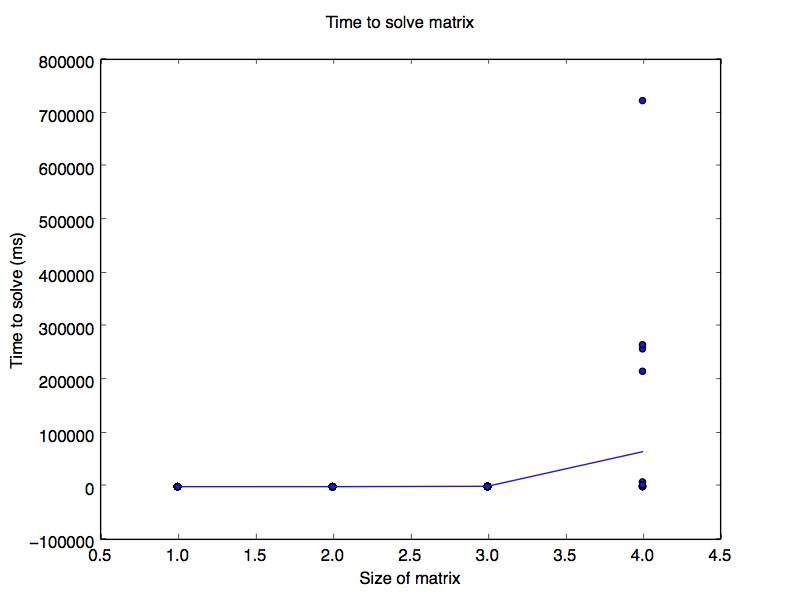
\includegraphics[]{src/allN.jpg}

\subsubsection{Application}
The proof above, for showing a runtime of $O(n^{2*n^4 + 2})$ is fairly straight forward but a runtime that is that exponential is horrible. To put in in perspective if it took 1 ms to calculate a sudoku for n = 1 then it would take 4 minutes to calculate a sudoku for n = 2, $2*10^70$ days to calculate a standard sudoku. Even though it does take a very long time for standard Sudoku it doesn't quite take this long. The reason is because even though the game tree is really really large, $n^{2*n^4}$ thanks to the reject subroutine we never need to search anywhere close to all of it. If we look at an empty sudoku game with no hints then at every box we have a very different branching factor that looks like:

\begin{center}
  \begin{tabular}{ | c | c | c | c | }
    \hline
    	4 & 3 & 2 & 1 \\ \hline
    	2 & 1 & 2 & 1 \\ \hline
    	2 & 2 & 1 & 1 \\ \hline
       	1 & 1 & 1 & 1 \\
    \hline
  \end{tabular}
\end{center}

Only one level actually has a $n^2$ branching factor the rest have a dramatic decrease. 

The same type of square can be shown for the $n = 3$ situation. 

\begin{center}
  \begin{tabular}{ | c | c | c | c | c | c | c | c | c |}
    \hline
    	9 & 8 & 7 & 6 & 5 & 4 & 3 & 2 & 1 \\ \hline
        7 & 6 & 5 & 6 & 5 & 4 & 3 & 2 & 1 \\ \hline
        3 & 2 & 1 & 3 & 2 & 1 & 3 & 2 & 1 \\ \hline
        6 & 5 & 4 & 6 & 5 & 4 & 3 & 2 & 1 \\ \hline
        5 & 4 & 3 & 6 & 5 & 4 & 3 & 2 & 1 \\ \hline
        3 & 2 & 1 & 3 & 2 & 1 & 3 & 2 & 1 \\ \hline
        3 & 2 & 1 & 3 & 2 & 1 & 3 & 2 & 1 \\ \hline
        2 & 2 & 1 & 2 & 2 & 1 & 2 & 2 & 1 \\ \hline
        1 & 1 & 1 & 1 & 1 & 1 & 1 & 1 & 1 \\ 
    \hline
  \end{tabular}
\end{center}

As we can see the branching factor is way better than the worst case proved above but it can not be generalized because the branching factor also depends on how many hints were given. 

\subsection{Space Complexity for size N}

\subsection{Space Complexity for Different Hints}

%---------------------------------------------------
\subsection{Runtime for constraints}

%---------------------------------------------------
\subsection{Inputs} 
\subsubsection{Inputs Worst Case}
\subsubsection{Inputs Average Case}
\subsubsection{Inputs Best Case}

 
\section{Conclusions}
I concluded stuff
%\end{document}  % This is where a 'short' article might terminate

%ACKNOWLEDGMENTS are optional
\section{Acknowledgments}
This section is optional; it is a location for you
to acknowledge grants, funding, editing assistance and
what have you.  In the present case, for example, the
authors would like to thank Gerald Murray of ACM for
his help in codifying this \textit{Author's Guide}
and the \textbf{.cls} and \textbf{.tex} files that it describes.

%
% The following two commands are all you need in the
% initial runs of your .tex file to
% produce the bibliography for the citations in your paper.
\cite{*}
\bibliographystyle{abbrv}
\bibliography{sigproc}  % sigproc.bib is the name of the Bibliography in this case
% You must have a proper ".bib" file
%  and remember to run:
% latex bibtex latex latex
% to resolve all references
%
% ACM needs 'a single self-contained file'!
%
%APPENDICES are optional
%\balancecolumns
\end{document}
